\documentclass{mathnotes}
\usepackage{mathnotes}

% % Necessary commands.
\newcommand{\thetitlename}{Ecuaciones en Derivadas Parciales}
\newcommand{\thetitle}{\HRule \thetitlename\\\HRule Notas no revisadas\footnote{Se agradecen sugerencias, correcciones, etc.}}
\newcommand{\theauthor}{Guillermo Ruiz Álvarez}
\newcommand{\thedate}{2015}

\begin{document}
\maketitle
\newpage
\tableofcontents
\newpage

\section{El principio del máximo}
\subsection{El principio del máximo unidimensional}

Esta sección comienza con el estudio del principio del máximo unidimensional en ecuaciones diferenciales.
\begin{mathresult}{Principio del máximo unidimensional}
Dada la inecuación 
\begin{equation}
\label{eq:principio-del-maximo}
-u''+g(x)u'+h(x)u(x) < 0 \ \ \forall x \in (0,1) 
\end{equation}
Si $h(x) \ge 0$ en el intervalo $(0,1)$, la solución de \eqref{eq:principio-del-maximo} no puede tener un máximo (local o global) no negativo en dicho intervalo.
\end{mathresult}
\begin{proof}
Sea $u$ la solución de \eqref{eq:principio-del-maximo}. Supongamos que $u$ tiene un máximo no negativo, es decir, $\exists c\in (0,1)$ que satisface $u(c) \ge u(x) \ \forall x \in (0,1)$ con $u(c)\ge 0$.
Si esto es así, la solución de la inecuación cumple $u'(c)=0$ y $u''(c) \le 0$. De aquí se obtiene:
$$\underbrace{-u''(c)}_{\ge 0}+\underbrace{g(c)u'(c)}_{=0}+\underbrace{h(c)u(c)}_{\ge 0} \ge 0$$
El tercer término es no negativo dado que, por hipótesis, $h(x) \ge 0$ en todo el intervalo y $u(c)$ es no negativo.
Esto nos lleva a una contradiccion con \eqref{eq:principio-del-maximo}, por tanto, $\nexists c \in (0,1)$ que satisfaga $u(c) \ge u(x) \ \forall x \in (0,1)$ con $u(c)\ge 0$.
\end{proof}
\see El resultado es cierto para cualquier intervalo abierto acotado, no sólo para $(0,1)$.

A partir del resultado anterior, se va a dar la prueba del siguiente teorema:

\begin{theorem}\label{theorem1}
Sea $u\in C^2(0,1)$ que satisface
\begin{equation}\label{eq:principio-del-maximo2}
-u''(x)+g(x)u'(x)+h(x)u(x) \le 0
\end{equation}
con $g, h$ acotadas y $h(x) \ge 0$ en cualquier subintervalo de $(0,1)$.

Entonces, si $\exists a\in (0,1)$ tal que $u(a) \ge u(x) \ \forall x\in(0,1)$ y $u(a) \ge 0$ (i.e. u alcanza un máximo no negativo en $a$), se tiene que $u = cte$ en $(0,1)$.
\end{theorem}
\begin{proof}
Sea $u$ la solución de \eqref{eq:principio-del-maximo2}. Supongamos que $u$ es una función no constante. Sabemos que $\exists b \in (0,1)$ tal que $u(b) < u(a)$ dado que $a$ es un máximo (local o global) de $u$ y $u$ es no constante. Supongamos $0< a < b < 1$.\footnote{Para el caso contrario la demostración es similar.}

Construimos la función
$$\varphi(x) = e^{\alpha(x-a)}-1$$

\begin{figure}[h]
\centering

\begin{tikzpicture}
	\draw[->] (-3,0) -- (3,0) node[right] {$x$};
	\draw[->] (0,-1) -- (0,3) node[above] {$y$};
	\draw[-]  (1, 0.1) -- (1, -0.1) node[below] {$a$};
	\draw[-]  (0.5, 0.1) -- (0.5, -0.1) node[below] {$\frac{a}{2}$};
	\draw[] (-0.2,0) node[below] {$0$};
	\draw[-]  (2, 0.1) -- (2, -0.1) node[below] {$1$};
	\draw[scale=1,domain=-1:2.3,smooth,variable=\x,blue] 
		plot ({\x},{exp(\x-1)-1})
		node[right] {$\varphi(x)$};
\end{tikzpicture}

\label{fig:phi-x}
\caption{Función $\varphi$}
\end{figure}

Si aplicamos \eqref{eq:principio-del-maximo2} a $\varphi$ obtenemos 

\begin{align*}
-\varphi''(x)+g(x)\varphi'(x)+h(x)\varphi(x) & \le 0 \numberthis \label{eq:phi-estricta}\\
e^{\alpha(x-a)}\left(-\alpha^2+\alpha g(x)\right) + h(x)\underbrace{(e^\alpha(x-a)-1)}_{\varphi} & \le 0\\
e^{\alpha(x-a)}\left(-\alpha^2+\alpha g(x)+\underbrace{h(x)}_{\ge 0}\underbrace{(1-e^{-\alpha(x-a)})}_{\le 1}\right) & \le 0\\
e^{\alpha(x-a)}\left(-\alpha^2 + \alpha g(x) + h(x)\right) & \le 0
\end{align*}

Dado que $g,h$ son acotadas, se puede tomar un valor de $\alpha$ suficientemente grande de forma que $-\alpha^2 + \alpha g(x) + h(x)  < 0$. Es decir, que $\varphi$ cumpla \eqref{eq:phi-estricta} para la desigualdad estricta. Tomamos $\alpha$ tal que la desigualdad estricta para $\varphi$ se cumpla $\forall x \in [\frac{a}{2}, b] \subset (0,1)$

Definimos ahora $$w(x) = u(x) + \varepsilon \varphi(x)$$
con $\varepsilon > 0$

Aplicando \eqref{eq:principio-del-maximo2} a $w$ obtenemos
\begin{align*}
-w'' + g(x)w'+h(x)w = & -u''+g(x)u'+h(x)u\\
& + \varepsilon\left(-\varphi''+g(x)\varphi'+h(x)\varphi\right)\\
\le &\ 0 + \varepsilon\left(-\varphi''+g(x)\varphi'+h(x)\varphi\right)\\
< &\ 0	\numberthis \label{eq:desigualdad-w}
\end{align*}
que se cumple $\forall x \in [\frac{a}{2}, b]$ si tomamos un valor de $\alpha$ adecuado. 
Dado que
\begin{equation*}
\left\{
\begin{array}{l}
w(b) = u(b) + \varepsilon\varphi(b)\\
w(a) = u(a)
\end{array}
\right.
\end{equation*}
 si tomamos $\varepsilon < \frac{u(a)-u(b)}{\varphi(b)}$ tenemos que 
 \begin{equation}\label{eq:wb-menor-wa}
 w(b) < w(a)
 \end{equation}
Además, como 
\begin{equation*}
\left\{
\begin{array}{l l}
w(a) = u(a) & \\
\varphi(x) < 0 & \forall x < a \\
\end{array}
\right.
\end{equation*}
tenemos que $w(x) = u(x) + \varepsilon\varphi(x) < u(x) < u(a) = w(a)$, 
es decir, 
\begin{equation}\label{eq:wx-menor-wa}
w(x) < w(a)
\end{equation}
en todo el intervalo $[\frac{a}{2}, a)$.

\noindent\textbf{Conclusión:}
\begin{itemize}
\item Utilizando \eqref{eq:desigualdad-w} y las hipótesis del teorema, obtenemos, para $w$, las hipótesis del \textbf{Principio del máximo}.
\item Vemos que $w$ tiene un máximo no negativo en el intervalo $[a, b)$, puesto que
\begin{itemize}
\item a la izquierda de $a$ tenemos \eqref{eq:wx-menor-wa}
\item a la derecha de $a$ tenemos \eqref{eq:wb-menor-wa}
\end{itemize}
Como $u$ es continua, tal y como está definida, $w$ también es continua. Se tiene entonces que $\exists c \in [a, b) \subset (\frac{a}{2}, b)$ tal que $w(c) = max\ w(x)$ en dicho intervalo. Es decir, $w$ alcanza un máximo no negativo, contradiciendo el teorema.
\end{itemize}
\newpage
Tenemos por tanto una contradicción, habiendo partido de las hipótesis del teorema y de la suposición de que $u$ es no constante.
\end{proof}

\corol
Sean $g,h$ acotadas y $u\in C[0,1] \cap C^2(0,1)$ una función no constante que satisface \eqref{eq:principio-del-maximo2}. 

Sea $M = \max_{x \in [0,1]}\ u(x)$. Sea $m = max\{u(0), u(1)\}$. Se tiene que:
\begin{itemize}
\item Si $M \ge 0 \implies u(x) < M\ \forall x\in(0,1)$
\item $u(x) < max\{0,m\}\ \forall x\in(0,1)$.
\end{itemize}

\begin{proof}
Dado que $[0,1]$ es un compacto y $u\in C[0,1]$, se tiene que $u$ alcanza un máximo $M$ en dicho intervalo.

\begin{itemize}
\item Caso $M<0$.

Como $M$ es un máximo de $u$, se cumple que $u(x) \le M < 0\ \forall x\in[0,1]$. Por tanto $u(x) < max\{0, m\}$.

\item Caso $M\ge 0$. 

Como $M$ es un máximo de $u$, se tiene que $m \le M$.

En las hipótesis del corolario tenemos que $u$ es no constante. Dado que $M$ es un máximo no negativo, no puede alcanzarse en el interior de $[0,1]$, porque si fuese así, por el teorema, $u$ sería constante. Así, el máximo se alcanza en $[0,1]\setminus(0,1)$ por lo que $m = M$.

Es decir, $u(x) < M = m = max\{0, m\}\ \forall x\in (0,1)$.
\end{itemize}
\end{proof}

Si suponemos, por ejemplo, que el máximo se alcanza en $x=0$. La solución de la ecuación, en un entorno de $0$, podría ser como se muestra en la figura \ref{fig:sol-entorno-cero}. Vamos a ver que condiciones son necesarias para que el caso de la figura \ref{fig:sol-entorno-cero-a}, en el que la tangente a la función es horizontal en el $0$, sea imposible.

\begin{figure}[ht]
\centering
\begin{subfigure}{.5\textwidth}
	\centering
  	\begin{tikzpicture}
		\draw[->] (-1,0) -- (3,0) node[right] {$x$};
		\draw[->] (0,-1) -- (0,3) node[above] {$y$};
		\draw[] (-0.2,0) node[below] {$0$};
		\draw[-, blue, dashed, scale=2] (0,1) -- (0.7,1);
		\draw[scale=2,domain=0:0.7,smooth,variable=\x,blue] 
			plot ({\x},{-(\x*\x)+1})
			node[right] {$u(x)$};
	\end{tikzpicture}
	\caption{}
	\label{fig:sol-entorno-cero-a}
\end{subfigure}%
\begin{subfigure}{.5\textwidth}
	\centering
  	\begin{tikzpicture}
		\draw[->] (-1,0) -- (3,0) node[right] {$x$};
		\draw[->] (0,-1) -- (0,3) node[above] {$y$};
		\draw[] (-0.2,0) node[below] {$0$};
		\draw[scale=2,domain=0:0.7,dashed,variable=\x,blue] 
			plot ({\x},{-0.4*\x+1});
		\draw[scale=2,domain=0:0.6,smooth,variable=\x,blue] 
			plot ({\x},{-(\x*\x)-0.4*\x+1})
			node[right] {$u(x)$};
	\end{tikzpicture}
	\caption{}
	\label{fig:sol-entorno-cero-b}
\end{subfigure}%

\caption{Función $u$ en un entorno de $0$}
\label{fig:sol-entorno-cero}
\end{figure}

\newpage
\begin{theorem}\label{theorem2}
Sea $u\in C^2(0,1)$ no constante que satisface \eqref{eq:principio-del-maximo2} y 
\begin{equation*}
\left\{
\begin{array}{l l}
u(0) \ge u(x) & \forall x \in (0,1)\\
u(0) \ge 0
\end{array}
\right.
\end{equation*}
es decir, $u$ alcanza un máximo no negativo en $0$.
Sea $h(x) \ge 0$.

Si $g(x) + xh(x)$ está acotada superiormente en un entorno de $0$, entonces
$$\lim_{x\to0^+}u'(x) < 0$$
\end{theorem}

\begin{proof}
Dado que $u$ es no constante $\exists a\in (0,1)$ tal que $u(a) < u(0)$.
Consideremos $\varphi(x) = e^{\alpha x}-1$. 

\begin{figure}[h]
\centering

\begin{tikzpicture}
	\draw[->] (-3,0) -- (3,0) node[right] {$x$};
	\draw[->] (0,-1) -- (0,3) node[above] {$y$};
	\draw[-]  (1, 0.1) -- (1, -0.1) node[below] {$a$};
	\draw[] (-0.2,0) node[below] {$0$};
	\draw[-]  (2, 0.1) -- (2, -0.1) node[below] {$1$};
	\draw[scale=1,domain=-1:1.3,smooth,variable=\x,blue] 
		plot ({\x},{exp(\x)-1})
		node[right] {$\varphi(x)$};
\end{tikzpicture}

\label{fig:phi2-x}
\caption{Función $\varphi$}
\end{figure}

Tenemos que
\begin{align*}
-\varphi''(x)+g(x)\varphi'(x)+h\varphi & = \\
e^{\alpha x}\left\{-\alpha^2 +\alpha g(x)+\underbrace{h(x)}_{\ge 0}\left(\underbrace{1-e^{-\alpha x}}_{\text{concava }(\le ax)}\right)\right\} & \le\\
e^{\alpha x}\left\{-\alpha^2+\alpha g(x) + \alpha xh(x)\right\} & = \\
\alpha e^{\alpha x}\{-\alpha + \left(\underbrace{g(x) +xh(x)}_{\text{acotado superiormente}}\right)\} & < 0
\end{align*}
es decir
$$-\varphi''(x)+g(x)\varphi(x)+h\varphi < 0$$
para un valor de $\alpha$ adecuado. Definimos ahora
$$w(x) = u(x) +\varepsilon \varphi(x)$$
Tenemos que
\begin{align*}
-w'' + g(x)w'+h(x)w = & -u''+g(x)u'+h(x)u\\
& + \varepsilon\left(-\varphi''+g(x)\varphi'+h(x)\varphi\right)\\
\le &\ 0 + \varepsilon\left(-\varphi''+g(x)\varphi'+h(x)\varphi\right)\\
< &\ 0
\end{align*}
Dado que $w(a) = u(a) + \varepsilon\varphi(a)$, si tomamos $\varepsilon < \frac{u(0)-u(a)}{\varphi(a)}$, se cumple que $w(a) < u(0) = w(0)$.
Tenemos por tanto que $w(a) \le w(x)\ \forall x \in [0, a]$. Obtenemos, $$\lim_{x\to0^+}w'(x) \le 0$$
Para ver la desigualdad estricta, basta con derivar $w$:
$$w'(x) = u'(x) +\varepsilon\varphi'(x)$$
Sabemos que $\varphi'(x) = \alpha e^{\alpha x}$, por tanto $\varphi'(0) = \alpha$.
Con esta información, tenemos
$$\lim_{x\to0^+} w(x) = \lim_{x\to0^+} u(x) +\varepsilon \alpha \le 0$$
Es decir, $$\lim_{x\to0^+} u(x) \le -\varepsilon \alpha < 0$$
\end{proof}

Vamos a ver la necesidad de que $g(x)$ y $g(x) + xh(x)$ sean acotadas para el teorema \ref{theorem1} y \ref{theorem2}, respectivamente. Veámoslo con un contraejemplo. Supongamos que
\begin{equation*}
g(x) = 
\left\{
\begin{array}{l l}
3/x & x\neq 0\\
0 & x = 0
\end{array}
\right.
\end{equation*}


\begin{figure}[ht]
\centering
\label{fig:g-de-x}
\begin{tikzpicture}
	\draw[->] (-3,0) -- (3,0) node[right] {$x$};
	\draw[->] (0,-3) -- (0,3) node[above] {$y$};
	\draw [fill, blue] (0,0) circle [radius=.05];
	\draw[scale=1,domain=-3:-1,smooth,variable=\x,blue] 
		plot ({\x},{3/(\x)});
	\draw[scale=1,domain=1:3,smooth,variable=\x,blue] 
		plot ({\x},{3/(\x)})
		node[right] {$g(x)$};
\end{tikzpicture}
\caption{Función $g$}
\end{figure}

Sea $u(x) = 1-x^4$ y $h(x) = 0$. Vemos que $u$ cumple
\begin{equation*}
\left\{
\begin{array}{l l}
-u''(x) + g(x)u'(x) = 0 & \forall x\in(-1,1)\\
u(0)=1 > u(x) & \forall x\in(-1,1)\\
\end{array}
\right.
\end{equation*}

Sin embargo, si observamos la figura \ref{fig:sol-contraejemplo-pm} vemos que no se cumplen ninguno de los dos teoremas anteriores.
\begin{itemize}
\item En el caso en el que consideremos la función en el intervalo $(-1,1)$, vemos que $u$ presenta un máximo no negativo en $(0,1)$. (Ver figura \ref{fig:sol-contraejemplo-pm1}). No se cumple el teorema \ref{theorem1} por no estar $g(x)$ acotada.
\item En el caso en el que consideremos la función en el intervalo $(0,1)$, vemos que $\lim_{x\to0^+}u(x) = 0$ (Ver figura \ref{fig:sol-contraejemplo-pm2}). No se cumple el teorema \ref{theorem2} por no estar $g(x)+xh(x)$ acotada.
\end{itemize}

\begin{figure}[ht]
\centering
\begin{subfigure}{.5\textwidth}
	\centering
  	\begin{tikzpicture}
		\draw[->] (-2,0) -- (2,0) node[right] {$x$};
		\draw[->] (0,-1) -- (0,1.5) node[above] {$y$};
		\draw[-] (-1,0.1) -- (-1,-0.1) node[below] {$-1$};
		\draw[-] (1,0.1) -- (1,-0.1) node[below] {$1$};
		\draw[scale=1,domain=-1:1,smooth,variable=\x,blue] 
			plot ({\x},{sqrt(1-\x*\x)})
			node[above right] {$u(x)$};
	\end{tikzpicture}
	\caption{}
	\label{fig:sol-contraejemplo-pm1}
\end{subfigure}%
\begin{subfigure}{.5\textwidth}
	\centering
  	\begin{tikzpicture}
		\draw[->] (-1,0) -- (2,0) node[right] {$x$};
		\draw[->] (0,-1) -- (0,1.5) node[above] {$y$};
		\draw[-, dashed, blue] (0,1) -- (1.5,1);
		\draw[] (-0.2,0) node[below] {$0$};
		\draw[-] (1,0.1) -- (1,-0.1) node[below] {$1$};
		\draw[scale=1,domain=0:1,smooth,variable=\x,blue] 
			plot ({\x},{sqrt(1-\x*\x)})
			node[above right] {$u(x)$};
	\end{tikzpicture}
	\caption{}
	\label{fig:sol-contraejemplo-pm2}
\end{subfigure}%

\caption{Función $u$}
\label{fig:sol-contraejemplo-pm}
\end{figure}

\newpage
\subsection{El principio del máximo n-dimensional}
\begin{mathresult}{Principio del máximo n-dimensional}
Dada la inecuación
\begin{equation}\label{eq:principio-del-maximo-Ndim}
-\Delta u(x) + \sum_{i=1}^n g_i(x)\frac{du(x)}{dx_i}+h(x)u(x) < 0 \ \ \forall x\in\Omega
\end{equation}

Sea $u\in C^2(\Omega)$ la solución de \eqref{eq:principio-del-maximo-Ndim}.
Si $h(x) \ge 0$, $u$ no puede alcanzar un máximo no negativo en $\Omega$.
\end{mathresult}
\see $\Delta u(x)$ es el laplaciano de $u(x)$ y se define como sigue:
$$\Delta u(x) = \sum_{i=1}^n\frac{d^2u(x)}{d^2x_i}$$

$\nabla u(x)$ es el gradiente de $u(x)$ y se define como sigue:
$$\nabla u(x) = \left(\frac{du(x)}{dx_1}, \hdots, \frac{du(x)}{dx_n}\right)^T$$
\begin{proof}
Sea $x_0\in \Omega$ y $u$ la solución de \eqref{eq:principio-del-maximo-Ndim}. Supongamos que $u$ alzanca un máximo no negativo en $x_0$, es decir, $u(x_0) \ge 0$ y $u(x_0) > u(x)\ \forall x \in \Omega$.

Definimos 
\begin{equation*}
\begin{array}{l r l l}
f: & (-\varepsilon, \varepsilon) \subset\mathbb{R} & \longrightarrow  & \mathbb{R}\\
& t & \longrightarrow & f(t) = u(x_0+t\xi)\\
\end{array}
\end{equation*}
con $\xi\in\mathbb{R}^n$.
Se puede observar que $f(0)$ es un máximo para $f$, por tanto
\begin{equation}
\left\{
\begin{array}{l}
f'(0) = 0\\
f''(0) \le 0\\
\end{array}
\right.
\end{equation}

Vamos a analizarlo por partes:
\begin{itemize}
\item $f'(0) = \nabla u(x_0)\xi$. Tenemos entonces que $\nabla u(x_0) = \vec{0}$
\item $f''(0) = \sum_{i,j=1}^n \xi_i\xi_j\frac{d^2u(x_0)}{dx_idx_j} = \xi^T\nabla^2u(x_0)\xi$. De donde se obtiene que $\nabla^2u(x_0) \le 0$. Es decir, $\nabla^2u(x_0)$ es semidefinida negativa.
\end{itemize}

Si tomamos $\xi_i = (0,\hdots, \underbrace{1}_{\text{posición i}}, \hdots, 0)^T$, obtenemos
$$\xi_i^T\nabla^2u(x_0)\xi_j = \Delta u(x_0)$$
Se tiene entonces que $\Delta u(x_0) \leq 0$.
Vamos a analizar ahora la inecuación en $x_0$:
\begin{equation}\label{eq:ineq-Ndimensional}
\underbrace{-\Delta u(x_0)}_{\ge 0} + \sum_{i=1}^n g_i(x_0)\underbrace{\frac{du(x_0)}{dx_i}}_{=0}+\underbrace{h(x_0)}_{\ge 0}u(x_0) \ge 0
\end{equation}

\noindent\textbf{Conclusión:}
Partiendo de las hipótesis del teorema, y suponiendo que $u(x_0)$ es un máximo no negativo, llegamos a \eqref{eq:ineq-Ndimensional}, que supone una contradicción con \eqref{eq:principio-del-maximo-Ndim}.
\end{proof}

\subsection{Principio débil del máximo}
\begin{mathresult}{Principio débil del máximo}
Dada la inecuación
\begin{equation}\label{eq:theorem3}
-\Delta u(x) + \sum_{i=1}^n g_i(x)\frac{du(x)}{dx_i}+h(x)u(x) \le 0 \ \ \forall x\in\Omega
\end{equation}
Sea $\Omega$ un \textbf{dominio} en $\mathbb{R}^n$.
Sea $u\in C(\overline{\Omega})\cap C^2(\Omega)$ la solución de \eqref{eq:theorem3}.
Sean $g_1,\hdots, g_n,h$ funciones acotadas.
Entonces:
\begin{itemize}
\item Si $h=0$ en $\Omega \implies \max_{\overline{\Omega}} u(x)$ se alcanza en $\delta\Omega$. 
\item Si $h>0$ en $\Omega \implies sup_{\Omega} u(x) \le max\left\{0, \max_{\delta\Omega} u(x)\right\}$. Es decir, $u$ no puede tener un máximo no negativo en $\Omega$.
\end{itemize}
\end{mathresult}
\newpage
\see
\begin{itemize}
\item Un \textbf{dominio} es un abierto conexo.
\item $\delta\Omega$ se refiere a la frontera de $\Omega$ 
\item $\overline{\Omega}$ al cierre (o adherencia) de $\Omega$.
\end{itemize}
\begin{proof}
\textbf{Caso $h = 0$}

Como $\Omega$ es un dominio, es acotado, (ver figura \ref{fig:omega}). Por tanto podemos suponer que está en una franja (una variable, por ejemplo $x_1$, se restringe). $\Omega \subset \{x\in \mathbb{R}^n: 0 < x_1 < d\}$.

\begin{figure}[ht]
\centering
\begin{tikzpicture}[scale=2]
\path [pattern=north west lines, pattern color=yellow] (0, -1.2) -- (0, 1.7) -- (2.5, 1.7) -- (2.5, -1.2);
\draw[->] (-1,0) -- (3,0) node[right] {$x_1$};
\draw[] (0,0) node[below left] {$0$};
\draw[] (2.5,0) node[below right] {$d$};
\draw [thick, fill=lemonchiffon] 
	(0.4,0) to [out=87,in=160] 
	(1.4,1) to [out=340,in=30]
	(2.25,.15) to [out=220,in=70]
	(1.4,0) to [out=273, in=273]
	(0.4,0);
\draw [->, dashed] (0, -1.2) -- (0, 1.7);
\draw [->, dashed] (2.5, -1.2) -- (2.5, 1.7);
\draw [] (1.3,1) node[below=3mm] {$\Omega$};

\end{tikzpicture}
\caption{Dominio $\Omega$}
\label{fig:omega}
\end{figure}
Consideramos la función $\varphi(x) = e^{\alpha x_1}$.
Si tomamos un valor de $\alpha$ suficientemente grande, tenemos:
\begin{equation}\label{eq:prueba1-ndim}
-\Delta\varphi + \sum_{i=1}^ng_i(x)\frac{d\varphi}{dx_i} = \alpha e^{\alpha x_1}\left(-\alpha + \underbrace{g_1(x)}_{\text{acotada}}\right) < 0
\end{equation}
Definimos ahora $w(x) = u(x) + \varepsilon\varphi(x)$, que cumple
\begin{align*}
-\Delta w + \sum_{i=1}^{n}g_i(x)\frac{dw}{dx_i} & \le\\
0 + \varepsilon\left(-\Delta\varphi + \sum_{i=1}^{n}g_i(x)\frac{d\varphi}{dx_i}\right) & \underbrace{<}_{\text{\eqref{eq:prueba1-ndim}}} 0
\end{align*}
A partir de la definición de $w$, dado que $\varepsilon, \varphi > 0$, se tiene que:

\begin{equation*}
\begin{array}{l l l l}
u(x) & < & u(x) + \varepsilon\varphi(x) & \\
u(x) & < & w(x) & \forall x \in \Omega\\
\end{array}
\end{equation*}
Como $w$ cumple las hipótesis del \textbf{Principio del máximo n-dimensional}

\begin{equation*}
\begin{array}{l l l}
w(x)_\Omega & < & \max_{\delta\Omega} w(x) \\
w(x)_\Omega & < &  w(c) = u(c) + \epsilon\varphi(c)
\end{array}
\end{equation*}
para algún $c\in\delta\Omega$. Más precisamente

\begin{equation*}
\begin{array}{l l l}
w(x)_\Omega & < & \max_{\delta\Omega}u(x) + \varepsilon e^{\alpha d}
\end{array}
\end{equation*}
Si $\varepsilon\to0$
$$u(x)_\Omega < \max_{\delta\Omega}u(x)$$
es decir, el máximo de la función se alcanza en la frontera de $\Omega$.

\noindent\textbf{Caso $h \ge 0$}

Sea $\Omega_+ = \{x\in \Omega: u(x) > 0\} \equiv$ abierto (ver figura \ref{fig:omega-mas}).

\begin{figure}[ht]
\centering
\begin{tikzpicture}[scale=2]
\draw [->, thick] (0.4, 1.1) -- (1.1, 0.5);
\path [fill=lemonchiffon] 
	(1.4,1) to [out=340,in=30]
	(2.25,.15) to [out=220,in=70]
	(1.4,0) to [out=190, in=130]
	(1.4,1);
\draw [thick] 
	(0.4,0) to [out=87,in=160] 
	(1.4,1) to [out=340,in=30]
	(2.25,.15) to [out=220,in=70]
	(1.4,0) to [out=273, in=273]
	(0.4,0);
\draw [dashed, thick]
	(1.4, 0) to [out=190, in=130]
	(1.4, 1) node[above] {$\delta\Omega\cap\Omega = \{x\in R^n: u(x) = 0\}$};
\draw [] (1.6,0.5) node[below] {$\Omega_+$};
\end{tikzpicture}
\caption{Dominio $\Omega$}
\label{fig:omega-mas}
\end{figure}

\noindent Sea $u$ la solución de 
\begin{equation*}
\begin{array}{l l}
-\Delta u + \sum_{i=0}^ng_i(x)\frac{du}{dx_i} + h(x)u(x)\le0 & \text{en } \Omega_+
\end{array}
\end{equation*}
por la definición de $\Omega_+$ y por ser $h(x) \ge 0$, se tiene $h(x)u(x) \ge 0$, por tanto, 

\begin{equation*}
\begin{array}{l l}
-\Delta u + \sum_{i=0}^ng_i(x)\frac{du}{dx_i} \le -h(x)u(x) \le 0 & \text{en } \Omega_+\\
-\Delta u + \sum_{i=0}^ng_i(x)\frac{du}{dx_i} \le 0 & \text{en } \Omega_+\\
\end{array}
\end{equation*}
En $\Omega_+$ se cumplen las hipótesis del primer apartado del teorema ($u$ cumple la inecuación cuando $h=0$), el cual ya se ha probado. Se tiene
$$\max_{\overline{\Omega}_+}u = \max_{\delta\Omega_+}u$$
y a partir de aquí
$$\max_{\delta\Omega_+}u \le \max_{\delta\Omega}u $$
En la parte de la frontera de $\Omega_+$ que está en $\Omega$ (la que aparece con línea discontinua en la figura \ref{fig:omega-mas}), $u$ es nula, resultando

\begin{equation*}
\left.
\begin{array}{l l}
\text{Si } x\in\overline{\Omega}_+ & 0\le u(x)\le \max_{\delta\Omega}\\
\text{Si } x\in\Omega\setminus\overline{\Omega}_+ & u(x) < 0
\end{array}
\right\}
u(x) \le \max\left\{0, \max_{\delta\Omega} u\right\}
\end{equation*}
\end{proof}

\see
A partir de aquí, se denotará
$$\mathcal{L}(u) = -\Delta u(x) + \sum_{i=1}^n g_i(x)\frac{du(x)}{dx_i} + h(x)u(x)$$
que es un funcional lineal:
\begin{itemize}
\item $\mathcal{L}(u+v) = \mathcal{L}(u) + \mathcal{L}(v)$
\item $\mathcal{L}(\lambda u) = \lambda\mathcal{L}(u)$
\end{itemize}

\newpage
\begin{mathresult}{Lema de Hopf}
Sea $\Omega$ un abierto de $R^n$ y $u\in C^2$ que satisface
\begin{equation*}
-\Delta u(x) + \sum_{i=1}^n g_i(x)\frac{du(x)}{dx_i} + h(x)u(x) \le 0 \ \text{en } \Omega
\end{equation*}
donde $g_1,\hdots,g_n,h$ son acotadas.
Sea $x_0$ un punto de la frontera de $\Omega$ que cumple:
\begin{itemize}
\item $u$ es continua en $x_0$.
\item $u(x_0) > u(x)\ \forall x\in\Omega$.
\item $u(x_0) \ge 0$.
\item \textbf{Condición de la esfera interior en $x_0$}: Hay una bola $B\subset\Omega$ con $x_0\in\delta B$.
\end{itemize}
Entonces, la derivada normal exterior de $u$ en $x_0$, si existe, satisface:
\begin{equation}
\frac{du(x_0)}{d\nu} > 0
\end{equation}
\end{mathresult}


\begin{figure}[ht]
\centering
\begin{tikzpicture}[scale=2]

\def \n {80} %Para omega
\def \m {10} %Para la bola

%Omega
\draw [thick] 
	(0, 1) to [out=80,in=160]
	(1.5, 1.3) to [out=340, in=90]
	(3, 1) to [out=270, in=340]
	(1.3, 0.7) to [out=160, in=260]
	(0, 1);

\begin{scope}
	%Scope de omega
	\clip
		(0, 1) to [out=80,in=160]
		(1.5, 1.3) to [out=340, in=90]
		(3, 1) to [out=270, in=340]
		(1.3, 0.7) to [out=160, in=260]
		(0, 1);
	%Recubrimiento de omega
	\foreach \s in {1,...,\n}
	{
	  \draw[-, ultra thin, gray] (\s/15,1.5) arc (100:200:1) ;
	}
	%Bola
	\draw [cadmiumorange] (1.35,1.25) ellipse (3mm and 2mm);
	
	\begin{scope}
		%Scope de la bola
		\clip (1.35,1.25) ellipse (3mm and 2mm);
		%Recubrimiento de la bola
		\foreach \s in {1,...,\m}
		{
	  		\draw[-, ultra thin, cadmiumorange] (\s/10+1.2, 1) -- (\s/10+0.2, 1.5);
		}
		\end{scope}
\end{scope}

%Vector nu
\draw [->, thick, red] (1.65,1.2) -- (1.70,1.6) node[above] {$\vec{\nu}$};

%Nodo x0
\draw [fill, blue] (1.65, 1.2) circle [radius=.02];
\draw [blue] (1.75, 1.4) node[left=1mm] {$x_0$};

%Nodo Omega
\draw [] (-0.2, 1.2) node[below] {$\Omega$};

%Nodo B
\draw [cadmiumorange] (1.7,1.25) node[above right] {$B$};
\end{tikzpicture}

\caption{Normal exterior de $u$ en $x_0$ sobre $\Omega$}
\label{fig:omega-hopf}
\end{figure}

\begin{proof}
Fijamos $\rho$ y $R$ de tal manera que $0<\rho<R$ y consideramos $$\varphi(x) = e^{-\alpha r^2} - e^{-\alpha R^2}$$
donde $r=|x-y|$ y $R$ es el radio de la bola $B$ que tiene a $x_0$ en su frontera (ver figuras \ref{fig:phi-hopf} y \ref{fig:bola-hopf}).

\begin{figure}[ht]
\centering
	\begin{subfigure}[b]{0.5\textwidth}
		\centering
		\begin{tikzpicture}
		\draw [->] (0,-0.5) -- (0,1.5);
		\draw [->] (-0.5, 0) -- (3,0) node[right] {$r$};
		\draw[scale=1.5,domain=0:2,smooth,variable=\x,blue] 
			plot ({\x},{exp(-\x*\x)-exp(-1)})
			node[right] {$\varphi(x)$};
		\draw[-] (1.5,0.1) -- (1.5,-0.1) node[below] {$R$};
		\draw[-] (0.7,0.1) -- (0.7,-0.1) node[below] {$\rho$};
		\end{tikzpicture}
		\caption{Función $\varphi$}
		\label{fig:phi-hopf}
	\end{subfigure}%
	\begin{subfigure}[b]{0.5\textwidth}
		\centering
		\begin{tikzpicture}
		\draw [fill, lightgray] (0, 0) circle [radius=2];
		\draw [fill, lightgrayminus] (0, 0) circle [radius=1];
		\draw [dashed] (0, 0) circle [radius=2];
		\draw [dashed] (0, 0) circle [radius=1];
		\draw [fill] (0, 0) circle [radius=0.05] node[below right] {$y$};
		\draw [-]  (0,0) -- (1,1.73) node[above right] {$x_0$};
		\draw [-] (0,0) -- (-0.5, 0.86) node[below=2mm] {$\rho$};
		\draw (0.9, 1.5) node[below] {$R$};
		\draw (0.9, -0.9) node[below] {$A$};
		\end{tikzpicture}
		\caption{Bola de centro $y$ y radio $R$}
		\label{fig:bola-hopf}
	\end{subfigure}
	\caption{}
\end{figure}

\noindent Calculamos
\begin{equation}\label{eq:hopfeq}
\mathcal{L}(\varphi) = -\Delta \varphi + \sum_{i=1}^n g_i(x)\frac{d\varphi}{dx_i} + h(x)\varphi
\end{equation}
Inicialmente tenemos
\begin{equation*}
\left\{
\begin{array}{l}
r^2 = \sum_{i=1}^n(x_i-y_i)^2\\
\frac{dr^2}{dx_i}=2(x_i-y_i)\\
\end{array}
\right.
\end{equation*}
A partir de aquí, recordando que $r = r(x) = |x-y|$:
\begin{itemize}
\item $\frac{d\varphi}{dx_i} = -2\alpha(x_i-y_i)e^{-\alpha r^2}$
\item $\frac{d^2\varphi}{d^2x_i} = e^{-\alpha r^2}\{-2\alpha-2\alpha(x_i-y_i)(-2\alpha(x_i-y_i)) \}$
\item $\Delta\varphi = \sum_{i=1}^n \frac{d^2y}{d^2x_i}= e^{-\alpha r^2}\{-2\alpha n+4\alpha^2r^2\}$
\end{itemize}
Sustituyendo en \eqref{eq:hopfeq}
\begin{equation*}
\begin{array}{r r}
\mathcal{L}(\varphi) = -\Delta \varphi + \sum_{i=1}^n g_i(x)\frac{d\varphi}{dx_i} + h(x)\varphi & = \\
e^{-\alpha r^2}\{-4\alpha^2r^2+2\alpha n-2\alpha x \cdot g(x)\} & + \\
\underbrace{h(x)}_{\ge 0}\{\underbrace{e^{-\alpha r^2}-e^{-\alpha R^2}}_{<e^{-\alpha r^2}}\} & \le \\
e^{-\alpha r^2}\{-4\alpha^2r^2+2\alpha n-2\alpha \underbrace{x \cdot g(x)}_{\text{acotado}} + \underbrace{h(x)}_{\text{acotado}}\} & < \\
e^{-\alpha \rho^2}\{-4\alpha^2\rho^2+2\alpha n-2\alpha x \cdot g(x) + h(x)\} & < 0 \\
\end{array}
\end{equation*}
en $A = B_R(y)\setminus \overline{B_\rho(y)}$ para un valor de $\alpha$ suficientemente grande. Pues en $A$, $r$ no se anula y por tanto el término que contiene $\alpha^2$ tampoco. Además, en $A$ se cumple que $\rho < r$.

Definimos ahora
$$w(x) = u(x) +\varepsilon\varphi(x)$$
que cumple
\begin{equation*}
\begin{array}{l r}
\mathcal{L}(w) = 0 + \varepsilon\mathcal{L}(\varphi) < 0 & \text{en } A
\end{array}
\end{equation*}
Utilizando el principio débil del máximo
$$w(x)_A < \max_{\delta A}w(x)$$
Por otro lado
$$w(x) \le \max u + \varphi(\rho) < u(x_0)$$
si $\varepsilon$ es lo suficientemente pequeño.
Dado que $w = u$ en $\delta B$
$$\max_{A} w(x) < \max_{\delta A} w = \max_{\delta B} w = w(x_0) = u(x_0)$$
De lo anterior tenemos que, si nos acercamos al máximo, la función es estrictamente creciente, lo que se traduce en
$$0\le\frac{dw(x_0)}{d\nu}$$
donde
$$\frac{dw(x_0)}{d\nu} = \frac{du(x_0)}{d\nu} + \varepsilon\underbrace{\varphi'(R)}_{<0}$$
Es decir,
$$\frac{du(x_0)}{d\nu} \ge -\varepsilon\varphi'(R) > 0$$
\end{proof}


\subsection{Principio fuerte del máximo}
\begin{mathresult}{Principio fuerte del máximo}
Sea $\Omega$ un dominio y $u\in C^2(\Omega)$ tal que $\mathcal{L} \le 0$ con $g_1,\hdots,g_n,h$ acotadas y $h\ge 0$.

\noindent Si $u$ alcanza un máximo no negativo en $\Omega$, entonces $u$ es constante.
\end{mathresult}

\begin{proof}
Supongamos que $u(x_0)$ es un máximo no negativo de $u$, con $x_0\in\Omega$.
Definimos $\Omega_{-}$ como sigue
$$\Omega_{-} = \{x\in\Omega: u(x) < u(x_0)\}$$
Si suponemos que $u$ es no constante, entonces $\Omega_{-}\neq \emptyset$. Además $x_0\in\delta\Omega_{-}\cap\Omega$


\begin{figure}[ht]
\centering

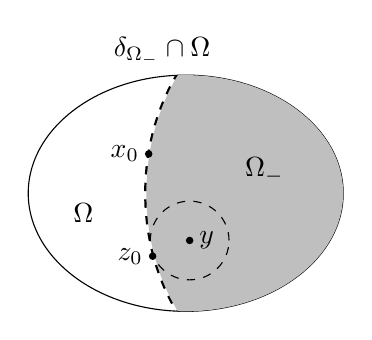
\begin{tikzpicture}
\draw (0,0) ellipse (2cm and 1.5cm);
\begin{scope}
	\clip (0,0) ellipse (2cm and 1.5cm);
	\draw [dashed, ultra thick] (1.5,0) ellipse (2cm and 	2.5cm);
	\path [fill, lightgray] (1.5,0) ellipse (2cm and 2.5cm);
\end{scope}
\draw [fill] (-0.47,0.5) circle [radius=0.4mm] node[left] {$x_0$};
\draw (-0.3,1.5) node[above] 
{$\delta_{\Omega_{-}}\cap \Omega$};
\draw (-1.3,-0.5) node[above] {$\Omega$};
\draw (1,0) node[above] {$\Omega_{-}$};
\draw [dashed] (0.05,-0.6) circle[radius=0.5cm];
\draw [fill] (0.05, -0.6) circle[radius=0.4mm] node[right] {$y$};
\draw [fill] (-0.42, -0.8) circle[radius=0.4mm] node[left] {$z_0$};
\end{tikzpicture}

\caption{$\Omega_{-}\subset\Omega$}
\label{fig:omegamenos}
\end{figure}

\noindent Vamos a tomar un $y\in\Omega$ de tal forma que $y$ esté más cerca de $\delta\Omega_{-}$ que de $\delta\Omega$ y consideramos la bola $B=B(y,R)$ con radio $R$ de tal manera que sea lo mayor posible para que quede dentro de $\Omega_{-}$ (ver figura \ref{fig:omegamenos}).
Llamamos $z_0$ a la intersección de $B$ con $\delta\Omega_{-}$.
Por como está definido $\Omega_{-}$ se puede observar que
$$\delta\Omega_{-}\cap\Omega = \{z\in\Omega: u(z) = u(x_0)\}$$
Así que $u(z_0) = u(x_0) \ge 0$.
Con todo esto, tenemos las hipótesis del \textbf{Lema de Hopf} para $\Omega_{-}$. Utilizando el lema se concluye que
$$\frac{du(z_0)}{d\nu} > 0$$
Como $\frac{du(z_0)}{d\nu} = \nabla u(z_0)\cdot \nu$. Por tanto $$\nabla u(z_0) \cdot \nu > 0\implies \nabla u(z_0) > 0$$
Sin embargo, al ser $u(z_0) = u(x_0)$ un máximo
$$\nabla u(z_0) = 0$$
Tenemos una contradicción al suponer que $u$ tiene un máximo no negativo y que es no constante.
\end{proof}
\newpage
\section{Problemas de condiciones de contorno}
Se denomina problema de condiciones de contorno al conjunto de una ecuación diferencial y datos iniciales en la frontera de una región.

\subsection{Problema de Dirichlet}
El problema de Dirichlet es un problema de valores de contorno que consiste en hallar la solución $u \in C^2(\Omega)\cap C(\overline{\Omega})$ a una EDP en un dominio $\Omega$ acotado de tal forma que:
\begin{equation*}
\text{Si }
\left.
\begin{array}{l}
F\in C(\Omega)\\
f\in C(\delta\Omega)
\end{array}
\right\}
\text{Se quiere hallar } u\text{ tal que }
\left\{
\begin{array}{l r}
\mathcal{L}(u) = F &\text{en } \Omega\\
u = f &\text{en } \Omega\\
\end{array}
\right.
\end{equation*}

\subsubsection{Unicidad}
\begin{prop}{Unicidad del problema de Dirichlet}
Si $\mathcal{L}(u)=\mathcal{L}(v)$ en $\Omega$ y $u=v$ en $\delta\Omega$ entonces $u = v$ en $\Omega$.
\end{prop}
\begin{proof}
Sea $w=u-v$. Como $\mathcal{L}$ es un funcional lineal, se tiene
$$\mathcal{L}(w) = \mathcal{L}(u-v) = \mathcal{L}(u)-\mathcal{L}(v) = 0-0 = 0$$
De las hipótesis se tiene que
\begin{equation*}
\left.
\begin{array}{l l}
\mathcal{L} = 0 & \text{en } \Omega\\
w = 0 & \text{en } \delta\Omega\\
\end{array}
\right\}
\max_{\Omega}w\le\max\{0,\max_{\delta\Omega}w\} = 0
\end{equation*}
es decir, $w\le0$ en $\Omega$. Al ser $\mathcal{L}$ lineal, si $w$ es solución, $-w$ también, por tanto se puede realizar el mismo proceso para llegar a que $-w\le0$ en $\Omega$.
$$w\le0 \wedge -w\le0 \iff w = 0$$
\end{proof}


\subsubsection{Comparación de soluciones}
\begin{prop}{Comparación de soluciones}
Si $\mathcal{L}(u) \le \mathcal{L}(v)$ en $\Omega$ y $u\le v$ en $\delta\Omega$, entonces $u\le v$ en $\Omega$.
\end{prop}
\begin{proof}
Sea $w = u-v$. 
Como $\mathcal{L}$ es un funcional lineal, se tiene
$$\mathcal{L}(w) = \mathcal{L}(u-v) = \mathcal{L}(u)-\mathcal{L}(v) \le 0$$
De las hipótesis se tiene que
\begin{equation*}
\left.
\begin{array}{l l}
\mathcal{L} \le 0 & \text{en } \Omega\\
w \le 0 & \text{en } \delta\Omega\\
\end{array}
\right\}
\max_{\Omega}w\le\max\{0,\max_{\delta\Omega}w\} = 0
\end{equation*}
es decir, $w \le 0$ en $\Omega$. De donde se obtiene que $u\le v$ en $\Omega$.
\end{proof}


\subsection{Problema de Neumann}
El problema de Neumann es un problema de valores de contorno que consiste en hallar la solución $u \in C^2(\Omega)\cap C^1(\overline{\Omega})$ a una EDP en un dominio $\Omega$ acotado de tal forma que:
\begin{equation*}
\text{Si }
\left.
\begin{array}{l}
F\in C(\Omega)\\
f\in C(\delta\Omega)
\end{array}
\right\}
\text{Se quiere hallar } u\text{ tal que }
\left\{
\begin{array}{l r}
\mathcal{L}(u) = F &\text{en } \Omega\\
\frac{du}{d\nu} = f &\text{en } \Omega\\
\end{array}
\right.
\end{equation*}

\subsection{Unicidad}
\begin{prop}{Unicidad del problema de Neumann}
Sean $u,v$ tales que satisfacen $\mathcal{L}(u)=\mathcal{L}(v)$ en $\Omega$ y $\frac{du}{d\nu} = \frac{dv}{d\nu}$ en $\delta\Omega$.
Si $h(x)\ge0$ en $\Omega$ y en todo punto de $\delta\Omega$ se tiene la \textbf{condición de la esfera interior}, entonces $u-v=cte$ en $\Omega$.
\end{prop}
\begin{proof}
Supongamos $w=u-v\neq cte$ en $\Omega$. Al ser $\overline{\Omega}$ un compacto, o bien $w$ o bien $-w$ tiene un máximo no negativo en algún punto $x_0$. Por el principio del máximo, $x_0\in\delta\Omega$.
Por hipótesis se tiene que $\frac{dw(x_0)}{d\nu} = 0$. Sin embargo, por el \textbf{lema de Hopf} $\frac{dw(x_0)}{d\nu} > 0$. Llegamos a una contradicción al suponer que $w=u-v\neq cte$ en $\Omega$.
\end{proof}
\see
\noindent Si $h(x) > 0$ en algún punto de $x\in\Omega$, entonces $u=v$.

\noindent Como $\mathcal{L}(u-v) = 0$, se tiene
$$\mathcal{L}(u-v) = -\Delta (u-v) + \sum_{i=1}^n g_i(x)\frac{d(u-v)}{dx_i} + h(x)(u-v) = 0$$
Pero $u-v=cte$, por lo que queda que
$$h(x)(u-v) = 0$$ Como $h(x)$ es estrictamente positiva, entonces $u-v=0$.

\example
Vamos a ver la necesidad de que $h(x)\ge 0$ en todo el dominio.
Se tiene la ecuación siguiente:
$$-u''-u=0$$
en la que $h(x) = -1 < 0$.
Dos soluciones de esta ecuación son
\begin{equation*}
\begin{array}{l}
u_1(x) = sin(x)\\
u_2(x) = cos(x)\\
\end{array}
\end{equation*}

\begin{figure}[ht]
\centering
\begin{subfigure}{.5\textwidth}
	\centering
  	\begin{tikzpicture}
		\draw[->] (-0.5,0) -- (4,0) node[right] {$x$};
		\draw[->] (0,-1) -- (0,1.5) node[above] {$y$};
		\draw[-] (pi/2,0.1) -- (pi/2,-0.1) node[below] {$\frac{\pi}{2}$};
		\draw[-] (pi,0.1) -- (pi,-0.1) node[below] {$\pi$};
		\draw[] (-0.2,0) node[below] {$0$};
		\draw[fill, blue] (pi/2, 1) circle[radius=0.5mm];
		\draw[scale=1,domain=0:pi,smooth,variable=\x,blue] 
			plot ({\x},{sin(\x r)})
			node[above right] {$u(x)$};
	\end{tikzpicture}
	\caption{$u(x) = sin(x)$}
	\label{fig:sol-contraejemplo-h1}
\end{subfigure}%
\begin{subfigure}{.5\textwidth}
	\centering
  	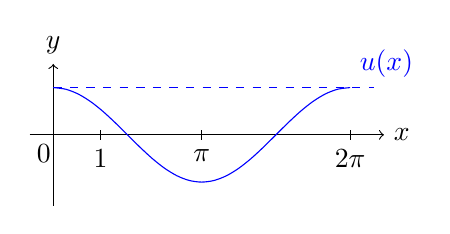
\begin{tikzpicture}[scale=0.6]
		\draw[->] (-0.5,0) -- (7,0) node[right] {$x$};
		\draw[->] (0,-1.5) -- (0,1.5) node[above] {$y$};
		\draw[-] (pi,0.1) -- (pi,-0.1) node[below] {$\pi$};
		\draw[-] (2*pi,0.1) -- (2*pi,-0.1) node[below] {$2\pi$};
		\draw[-, dashed, blue] (0,1) -- (2*pi+0.5,1);
		\draw[] (-0.2,0) node[below] {$0$};
		\draw[-] (1,0.1) -- (1,-0.1) node[below] {$1$};
		\draw[scale=1,domain=0:2*pi,smooth,variable=\x,blue] 
			plot ({\x},{cos(\x r)})
			node[above right] {$u(x)$};
	\end{tikzpicture}
	\caption{$u(x) = cos(x)$}
	\label{fig:sol-contraejemplo-h2}
\end{subfigure}%
\caption{Funciones periódicas}
\label{fig:sol-contraejemplo-h}
\end{figure}

\noindent En la figura \ref{fig:sol-contraejemplo-h1} se puede ver como se alcanza un máximo no negativo en el interior del invervalo. En la figura \ref{fig:sol-contraejemplo-h2} se observa como la función llega a los extremos del intervalo con derivada nula. Ambas situaciones se deben a que no se cumple la condición $h(x) \ge 0$.

\example
Vamos a ver la necesidad de que $\Omega$ sea un dominio acotado.
Sean $u(x,y) = e^xsin(x)$ y $\Omega = \mathbb{R}\times(0, \pi)$
Se tiene que 
\begin{equation*}
u \text{ cumple}
\left\{
\begin{array}{l l}
-\Delta u = 0 & \text{en }\Omega\\
u=0 & \text{en } \delta\Omega\\
\end{array}
\right.
\end{equation*}
\begin{equation*}
\delta\Omega = (\mathbb{R}\times\{0\})\cup(\mathbb{R}\times\{\pi\})
\end{equation*}
Dado que $u(x) = 0$ en toda la frontera, se tiene que cumplir que $u(x) \le 0$ en $\Omega$, sin embargo, esto es falso por no ser $\Omega$ acotado (ver figura \ref{fig:u3d1}).

\begin{figure}[ht]
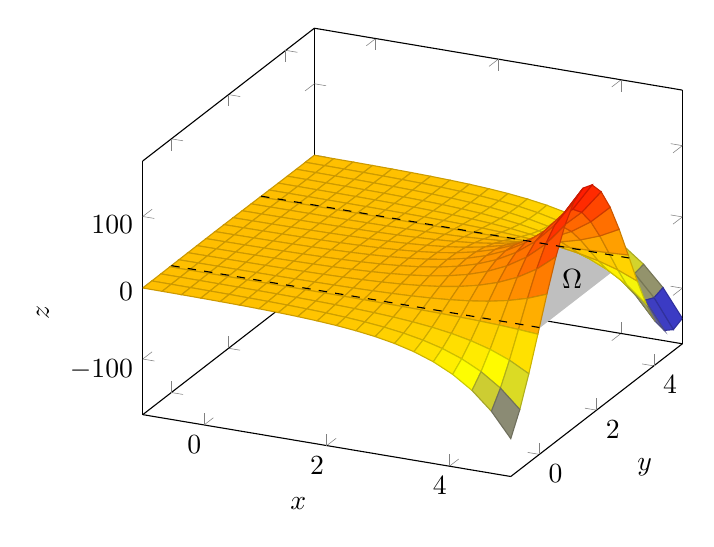
\begin{tikzpicture}
\begin{axis}[
	xlabel=$x$,
	ylabel=$y$,
	zlabel=$z$
]

\addplot3 [color=lightgray, fill] coordinates {(-1,pi,0) (5,pi,0) (5,0,0) (-1,0,0)};

\addplot3[
	surf,
    domain=-1:5,
    samples=20,
	] {(exp(\x))*sin(\y r)};

\addplot3 [color=black, dashed] coordinates {(-1,0,0) (5,0,0)};
\addplot3 [color=black, dashed] coordinates {(-1,pi,0) (5,pi,0)};
\node at (axis cs:4.6,2,0) {$\Omega$};
\end{axis}
\end{tikzpicture}
\caption{$u(x,y) = e^xsin(y)$}
\label{fig:u3d1}
\end{figure}

\newpage
\begin{theorem}
Sea $\Omega$ un dominio acotado, $u\in C^2(\Omega)\cap C(\overline{\Omega})$. 
Sea la inecuación
$$\mathcal{L}(u) \le F  \text{ en } \Omega\\$$
Si $g_1,\hdots,g_n,h$ son acotadas y $h(x) \ge 0$ entonces,
$$u(x) \le \max\{0, \max_{\delta\Omega}u\} + C\max\{0, \max_{\Omega} F\}$$
con $C$ una constante que depende del dominio $\Omega$ y de $g_1,\hdots,g_n$.
\end{theorem}
\begin{proof}
Se va a denotar
\begin{equation*}
\left\{
\begin{array}{l}
\mathcal{L}_0(u)=-\Delta u+\sum_{i=0}^ng_i(x)\frac{du}{dx_i}\\
\mathcal{L}(u) = \mathcal{L}_0(u)+h(x)u\\
M=\max\{0,\max_{\delta\Omega}u\}
\end{array}
\right.
\end{equation*}
Dado que $\Omega$ es un dominio acotado, se tiene que
$\Omega\subset\{x\in\mathbb{R}^n: 0<x_1<d\}$ para algún $d\in\mathbb{R}$.
Definimos $\varphi(x)$ siendo $K$ una constante positiva.
$$\varphi(x)=K\left(e^{\alpha d}-e^{\alpha x_1}\right)+M > M \ge 0$$
Calculamos $\mathcal{L}_0(\varphi)$:
$$\mathcal{L}_0(\varphi)=-Ke^{\alpha x_1}\{-\alpha^2+\alpha \underbrace{g_1(x)}_{\text{acotada}}\}>Ke^{\alpha x_1} > K > 0$$
si tomamos un valor de $\alpha$ lo suficientemente grande.

\noindent Definimos ahora $w=u-\varphi$ y calculamos $\mathcal{L}(w)$:
$$\mathcal{L}(w) = \mathcal{L}(u)-\mathcal{L}(\varphi) \le F - \mathcal{L}_0(\varphi)-\underbrace{h(x)\varphi(x)}_{\ge0}<F(x)-K \le 0$$
Basta tomar $K=\max\{0, \max_{\Omega}F\}$ para tener $\mathcal{L}(w) < 0$.
Por otro lado se tiene que $u\le M$, por tanto $u-\varphi\le M - M = 0$. Es decir, $u \le \varphi$. Entonces 
$$u_\Omega \le \varphi_\Omega\implies u_\Omega \le K\max_\Omega\left(e^{\alpha d}-e^{\alpha x_1}\right) + M = K\left(e^{\alpha d}-1\right) + M$$
\textbf{Conclusión:}

Denotamos $C = \left(e^{\alpha d}-1\right)$. Se puede observar que $C$ depende de $\alpha$ y $d$, es decir, que depende ensencialmente del dominio y de la cota de las funciones $g_1,\hdots,g_n$.
Se tiene entonces que 
$$u(x) \le \max\{0, \max_{\delta\Omega}u\} + C\max\{0, \max_{\Omega} F\}$$
\end{proof}

\newpage
\appendix
\documentclass[nochap]{apuntes}
\title{Métodos numéricos para EDO}
\author{Pedro Valero}
\date{20-09-2015}

% Paquetes adicionales
\usepackage{tikztools}
\usepackage{fastbuild}
\usetikzlibrary{arrows}

\begin{document}
%\maketitle
\pagestyle{plain}

%%%%%%%%%%%%%%%%%%%%%%%%%%%%%%%%%%%%%%%%%%%%%%%%%%%%%%%%%%
%%
%%         HOJA 1
%%         Problema 5
%%
%%%%%%%%%%%%%%%%%%%%%%%%%%%%%%%%%%%%%%%%%%%%%%%%%%%%%%%%%%
\textbf{Deducir cuál es la procedencia de los coeficientes empleadas pen la fórmula de $y_{n+1}$ en el método Runge-Kutta de cuarto orden}

Los métodos de Runge-Kutta consisten en la estimación de la función $y(x)$ mediante la recursión:
\[y_{n+1} = y_n+ h \sum_{i=1}^s b_i K_i\]
donde
\[K_i = f\left(x_n+c_ih, y_n+h \sum_{j=1}^ia_{ij}K_j\right)\]

En concreto, el método Runge-Kutta de cuarto orden consiste en el empleo de la fórmula:
\[y_{n+1} = y_n +\frac{h}{6}(K_1+2K_2+2K_3+K_4)\]
siendo:
\[
\begin{array}{ll}
K_1 = & f(x_n,y_n)\\
K_2 = & f(x_n+\frac{h}{2}, y_n+\frac{h}{2}K_1)\\
K_3 = & f(x_n+\frac{h}{2}, y_n + \frac{h}{2}K_2)\\
K_4 = & f(x_n+h, y_n + h K_3)
\end{array}
\]

La idea del método es que la fórmula dada para $y_{n+1}$ coincida con el desarrollo de Taylor de esta función.

Puesto que tenemos que determinar 4 variables: $b_i|_1^4$, parece razonable escribir el desarrollo de Taylor de orden 4 de $y_{n+1}$ así como los desarrollo de Taylor de orden tres de las $K_i$ a fin de poder establecer una relación.


Empezaremos calculando los desarrollos de Taylor de orden 3 de los $K_i$ en torno a $x_n$:

\[K_1 = f(x_n,y_n)\]

\begin{remark}
A partir de ahora, para abreviar, escribiremos $g()$ para representar $g(x_n,y_n)$, sea cual sea la función $g$
\end{remark}

\[K_2 = f\left(x_n+\frac{h}{2},y_n+\frac{h}{2}K_1\right)=f()+f_x()\frac{h}{2}+f_y()\frac{h}{2}K_1 +\]
\[+ \frac{1}{2}\left( f_{x^2}()\left(\frac{h}{2}\right)^2 +2 f_{xy}()\frac{h}{2}\frac{h}{2}K_1 +f_{y^2}()\left(\frac{h}{2}K_1\right)^2\right) +\]
\[+   \frac{1}{6}\left( f_{x^3}()\left(\frac{h}{2}\right)^3 + 3f_{x^2y}\left(\frac{h}{2}\right)^2\frac{h}{2}K_1 + 3f_{xy^2}\frac{h}{2}\left(\frac{h}{2}K_1\right)^2 + f_{y^3}\left(\frac{h}{2}K_1\right)^3\right)\]

Si sustituimos ahora $K_1$ por su valor obtenemos:
\[K_2 = f\left(x_n+\frac{h}{2},y_n+\frac{h}{2}K_1\right)=f()+f_x()\frac{h}{2}+f_y()\frac{h}{2}f() +\]
\[+ \frac{1}{2}\left( f_{x^2}()\left(\frac{h}{2}\right)^2 +2 f_{xy}()\frac{h}{2}\frac{h}{2}f() +f_{y^2}()\left(\frac{h}{2}f()\right)^2\right) +\]
\[+   \frac{1}{6}\left( f_{x^3}()\left(\frac{h}{2}\right)^3 + 3f_{x^2y}\left(\frac{h}{2}\right)^2\frac{h}{2}f() + 3f_{xy^2}\frac{h}{2}\left(\frac{h}{2}f()\right)^2 + f_{y^3}\left(\frac{h}{2}f()\right)^3\right)\]

A fin de simplificar un poco la notación vamos a definir:
\[\begin{array}{l}
Df = f_x+f_yf\\
D^2f = f_{x^2}+2ff_{xy}+f_{y^2}f^2\\
D^3f = f_{x^3} + 3f_{x^2y}f + 3f_{xy^2}f^2 + f_{y^3}f^3
\end{array}\]

Con esta nueva notación, podemos reescribir $K_2$ como sigue:
\[K_2 = f() + \frac{h}{2}Df + \frac{h^2}{8}D^2f + \frac{h^3}{48}D^3f\]

Vamos ahora a por $K_3$

\[K_3 = f\left(x_n+\frac{h}{2},y_n+\frac{h}{2}K_2\right)=f()+f_x()\frac{h}{2}+f_y()\frac{h}{2}K_2 +\]
\[+ \frac{1}{2}\left( f_{x^2}()\left(\frac{h}{2}\right)^2 +2 f_{xy}()\frac{h}{2}\frac{h}{2}K_2 +f_{y^2}()\left(\frac{h}{2}K_2\right)^2\right) +\]
\[+   \frac{1}{6}\left( f_{x^3}()\left(\frac{h}{2}\right)^3 + 3f_{x^2y}\left(\frac{h}{2}\right)^2\frac{h}{2}K_2 + 3f_{xy^2}\frac{h}{2}\left(\frac{h}{2}K_2\right)^2 + f_{y^3}\left(\frac{h}{2}K_2\right)^3\right)\]

Ahora sustituimos $K_2$ por el valor que hemos calculado anteriormente, apoyándonos en la nueva notación definida siempre que sea posible y teniendo en cuenta que estamos manipulando el polinomio de taylor de orden 4 y, por tanto, todos los términos con potencia de $h$ superior a la cuarta desaparecerán.

Así tenemos
\[K_3 =f()+f_x()\frac{h}{2}+f_y()\frac{h}{2}\left( f()+\frac{h}{2}Df + \frac{h^2}{8}D^2f\right) +\]
\[+ \frac{1}{2}\left( f_{x^2}()\left(\frac{h}{2}\right)^2 +2 f_{xy}()\frac{h}{2}\frac{h}{2}\left(f() + \frac{h}{2}Df \right) +f_{y^2}()\left(\frac{h²}{4}f^2()+\frac{h^3}{4}f()Df\right)\right) +\]
\[+\frac{1}{6}\left( f_{x^3}()\left(\frac{h}{2}\right)^3 + 3f_{x^2y}\left(\frac{h}{2}\right)^2\frac{h}{2}f()+ 3f_{xy^2}\frac{h}{2}\left(\frac{h}{2}f()\right)^2 + f_{y^3}\left(\frac{h}{2}f()\right)^3\right)\]

Agrupando los térmnos llegamos a que
\[K_3 = f()+\left(\frac{h}{2}+f_y()\frac{h^2}{4}+\underbrace{2f_{xy}()\frac{h^3}{8}+f_{y^2}()\frac{h^3}{4}f()}_{\frac{h^3}{4}Df_y}\right)Df+\left(\frac{h^2}{8} + f_y\frac{h^3}{16}\right)D^2f +\left(\frac{h^3}{48}\right)D^3f\]

Por último, nos queda
\[K_4 = f\left(x_n+h,y_n+hK_3\right)=f()+f_x()h+f_y()hK_3 +\]
\[+ \frac{1}{2}\left( f_{x^2}()h^2 +2 f_{xy}()hhK_3 +f_{y^2}()\left(hK_3\right)^2\right) +\]
\[+   \frac{1}{6}\left( f_{x^3}()h^3 + 3f_{x^2y}h^2hK_3 + 3f_{xy^2}h\left(hK_3\right)^2 + f_{y^3}\left(hK_3\right)^3\right)\]

De nuevo, sustituimos $K_3$ por su valor, teniendo en cuenta que no nos interesan aquellos términos con potencia en $h$ mayor a 4 lleganod a:
\[K_4 = f()+f_x()h+f_y()h\left( f()+\left(\frac{h}{2}+f_y()\frac{h^2}{4}\right)Df + \frac{h^2}{8}D^2f\right) +\]
\[+ \frac{1}{2}\left( f_{x^2}()h^2 +2 f_{xy}()hh\left(f()+\frac{h}{2}Df\right) +f_{y^2}()\left(hf()\right)^2\right) +\]
\[+   \frac{1}{6}\left( f_{x^3}()h^3 + 3f_{x^2y}h^3f() + 3f_{xy^2}h\left(hf()\right)^2 + f_{y^3}\left(hf()\right)^3\right)\]

Agrupando los términos llegamos a que:
\[K_4 = f() + \left(h +f_yh\left(\frac{h}{2}+f_y()\frac{h^2}{4} \right)+f_{xy}\frac{h^3}{2}\right)Df + \left( \frac{h^2}{2} + f_y()\frac{h^3}{8}+\right) D^2f + \left( \frac{h^3}{6}\right) D^3f\]
\textcolor{red}{Se que la ecuación superior no es correcta pero no encuentro el problema}

De donde podemos simplificar aún más escribiendo
\[K_4 = f() + \left(h +f_y\frac{h^2}{2}+\left(\frac{h^3}{2}\right)Df_y + \frac{h^3}{4}f_y^2\right)Df + \left( \frac{h^2}{2} + f_y()\frac{h^3}{8}+\right) D^2f + \left( \frac{h^3}{6}\right) D^3f\]

Vamos a calcular el desarrollo de taylor de orden 4 de $y_{n+1}$.
\[y_{n+1} = y(x_{n+1}) = y(x_n) +h y'(x_n)+\frac{h^2}{2}y''(x_n)+\frac{h^3}{6}y'''(x_n) + \frac{h^4}{24}y''''(x_n)= \]
\[=  y_n + h f()+\frac{h^2}{2}\left(f_x()+f_y()\underbrace{f()}_{y_n'}\right)  + \]
\[+\frac{h^3}{6}\left(f_{x^2}()+2f_{xy}()f()+f_x()f_y()+f_{y^2}()f()+f_{y}()f_y()f() \right) +\]
\[ + \frac{h^4}{24} \left(f_{x^3}()+3()ff_{x^2y}()+f^3f_{y^3}()+f_y()(f_{x^2}()+2f()f_{zy}()+f^2()f_{y^2}())+3f_x()f_{xy}()+\]
\[+3f()f_y()f_{xy}()+3f^2()f_y()f_{y^2}()+3f^2()f_y()f_{y^2}()+f_x()f_y^2()+f()f_y^3())\right)\]

Ahora procedemos a reescribir $y_{n+1}$ con la nueva notación empleada al simplificar los $K_i$.

Así nos queda que
\[y_{n+1}=y_n+hf() + \frac{h^2}{2}Df+\frac{h^3}{6}\left(D^2f+f_yDf\right) + \frac{h^4}{24}\left( D^3f+3DfDf_y+f_yD^2f+f_y^2Df\right)\]
\textcolor{red}{Se que la ecuación superior no es correcta pero no encuentro el problema}

Ahora debemos igualar los coeficientes del polinomio de taylor en los dos desarrollos planteados de $y_{n+1}$, es decir, el mostrado en el párrafo superior y el obtenido al combinar las $K_i$ según la ecuación $y_{n+1} = y_n + aK_1+bK_2+cK_3+dK_4$. Con esto llegamos al sistema de ecuaciones:
\small
\[
(a+b+c+d)f= 6\cdot f \iff a+b+c+d = 6 \]
\[\frac{b}{2}Df + \frac{c}{2}Df + dDf= 6\cdot Df  \iff b+c+2d = 12\]

\[\frac{b}{8}D^2f +\frac{c}{4}f_y()Df+\frac{c}{8}D^2f + \frac{d}{2}f_yDf+\frac{d}{2}D^2f= 6D^2f+6f_yDf \]
\[\frac{b}{48}D^3f + \frac{c}{4}Df_yDf+\frac{c}{16}f_yD^2f+\frac{c}{48}D^3f+\frac{d}{4}f^2_yDf+\frac{d}{8}f_yD^2f + \frac{d}{6}D^3f= 6D^3f+18DfDf_y+6f_yD^2f+6f_y^2Df\]
\normalsize
Podemos ver cada ecuación como un polinomio donde las combinaciones de $D^if$ son las variables. Para que se de la igualdad, los coeficientes de cada forma de ese tipo deben coincidir. Aplicando esta regla, descomponemos el sistema de ecuaciones anterior en:
\[\begin{array}{l}
a+b+c+d=6\\
b+c+2d = 12\\
b+c+4d=48 \\
c+2d = 24\\
b+c+8d = 288\\
c = 72 \\
c +2d = 96 \\
d = 24
\end{array}\]

%\[
%\b%egin{array}{ll}%
%K_%1 = & f(x_n+c_1h,y_n)\\%
%K_%2 = & f(x_n+c_2h, y_n+a%_{21}K_1)\\%
%K_%3 = & f(x_n+c_3h, y_n +% a_{31}K_1+%a_{32}K_2)\\%
%K_%4 = & f(x_n+c_4h, y_n +% a_{41}K_1+%a_{42}K_2+a_%{43}K_3)%
%\e%nd{array}%
%\]%
%si%endo
%\[%y_{n+1}=y_n+h\left(α_1K_1+α_2K_2+α_3K_3+α_4K_4\right)\]%
%
%Nuestro objetivo ahora es determinar los valores $a_{ij}$, $α_k$ que hacen que la %fórmula dada para $y_{n+1}$ coincida con su desarrollo de taylor.%
%
%Empezaremos manipulando las $K_i$ para escribirlas como desarroll%os de taylor de la %función $f(x_n,y_n)$ de grado 3, para finalmente igualar la fórmu%la de $y_{n+1}$ con% %su desarrollo de taylor de orden 4.%
%
%Para simplificar la notación, escribiremos $\text{algo}()$ para representar $\text{%algo}(x_n,y_n)$, es decir, suprimiremos los argumentos de las funciones. %Además, %por simplificar las fórmulas que irán apareciendo a continuación, definimos los %siguientes operadores diferenciales:%
%
%%\[\begin{array}{ll}%
%%Df = & f_x+ff_y%
%%D^2f = & f_{xx}%+2ff_{xy}+f^2f_{yy}%
%%D^3f = & f_{xxx%}+3ff_{xxy}+3f^2f_{x%yy}+f^3f_{yyy}
%%\end{array}\]%
%\begin{remark}%
%Evaluar el pol%inomio de Taylor e $(x%_n,y_n)$ implica que estamos calculando el %polinomio en t%orno a $h=0$%
%\end{remark}%
%\small%
%\begin%{itemi%ze}
%\item %\textb%f{$K_1 =  f(x_n+c_1h,y_n)$}%
%
%\[K_1 = f(x_n+c_1h, y_n)=f()+c_1hf_x()+\frac{(c_1h)^2}{2}f_{x^2}()\]
%\textbf{Con esto ya hemos deducido la fórmula de $K_1$}
%
%\item \textbf{$K_2 =  f(x_n+c_2h, y_n+a_{21}K_1)$}
%
%\[K_2 = f(x_n+c_2h, y_n+a_{21}K_1) = f()+c_2hf_x()+a_{21}K_1f_y()+ \frac{1}{2}\left( %2(a_{21}K_1)f_{yx}()+(c_2h)^2f_{x^2}()\atop+(a_{21}K_1)^2f_{y^2}()\right)\]%
%
%\item \textbf{$K_3 =  f(x_n+c_3h, y_n + a_{31}K_1+a_{32}K_2)$}%
%\[K_3 = f(x_n+c_3h, y_n+a_{31}K_1+a_{32}K_2) = f() + c_3hf_x()+(a_{31}K_1+a%_{32}K_2)%f_y()+ \atop\frac{1}{2}\left( 2(a_{31}K_1+a_{32}K_2)f_{yx}()+(c_3h)^2f_{x^2%}()+(a_{3%1%}K_1+a_{32}K_2)^2f_{y^2}()\right)\]%
%
%\item \textbf{$K_4 =  f(x_n+c_4h, y_n + a_{41}K_1+a_{42}K_2+a_{43}K_3$)}
%\[K_4 = f(x_n+c_4h, y_n+(a_{41}K_1+a_{42}K_2+a_{43}K_3)) = f() + c_4hf_x()+(a_{41}%K_1+a_{42}K_2+a_{43}K_3)f_y() \atop+\frac{1}{2}\left( 2(c_4h+(a_{41}K_1+a_{42}K_2+%a_{%43}K_3))f_{yx}()+(c_4h)^2f_{x^2}()+((a_{41}K_1+a_{42}K_2+a_{43}K_3))^2f_{y^2}()\ri%ght%)\]%
%\en%d{itemize}
%\no%rmalsize
%
%Por otro lado tenemos que $y_{n+1}$ podrá expresarse como:
%\[y_{n+1} = y(x_{n+1}) = y(x_n) +h y'(x_n)+\frac{h^2}{2}y''(x_n)+\frac{h^3}{6}y'''(%x_n)= \atop y_n + h f(x_n,y_n)+\frac{h^2}{2}\left(f_x(x_n,y_n)+f_y(x_n,y_n)\%underbrace{f(x_n,y_n)}_{y_n'}\right)  + \]%
%\[+\frac{h^3}{6}\left( f_{x^2}(x_n,y_n)+2f%_{xy}(x_n,y_n)f(x_n,y_n)+f_{y^2}(x%_n,y_n)f(%x_n,y_n)^2\right) \]%
%
%Lo primero que podem%os comprobar es el coeficiente del término $h$ del desarrollo de %Taylor de $y_{n+1}$ %es $f(x_n,y_n)$.%
%
%Por otro lado, cuando sustituyamos las $K_i$ por sus respectivas fórmulas en la %ecuación $y_{n+1}=y_n+h\left(α_1K_1+α_2K_2+α_3K_3+α_4K_4\right)$, el coeficiente% del %término $h$ será $(α_1+α_2+α_3+α_4)f(x_n,y_n)$, de donde podemos deducir la ecua%ción:
%\begin{eqnarray}%
%α_1+α_2+α_3+α_4 %= 1%
%\end{eqnarray}%
%
%Veamos ahora cuales serán los coeficientes de $h^2$ en los dos desarrollos de $y_{n+1%}$ para poder establecer una relación:%
%\begin{eqnarray}%
%\frac{1}{2}\left(f_x(x_n,y_n)+f_y(x_n,y_n)\underbrace{f(x_n,y_n)}_{y_n'}\right) = \%frac{c_1}{2}f_{x^2}()(1+a_{21}f_y+a_{21}f_{xy}+)+
%\end{eqnarray}

\end{document}


\end{document}